% Intended LaTeX compiler: pdflatex
\documentclass[10pt,a4paper,UTF8]{article}
\usepackage{zclorg}
\usepackage{tikztheorem}
\author{张朝龙}
\date{}
\title{自伴算子和正规算子}
\hypersetup{
 pdfauthor={张朝龙},
 pdftitle={自伴算子和正规算子},
 pdfkeywords={},
 pdfsubject={},
 pdfcreator={Emacs 25.2.1 (Org mode 9.0.9)},
 pdflang={English}}
\begin{document}

\maketitle
\tableofcontents
\titlepic{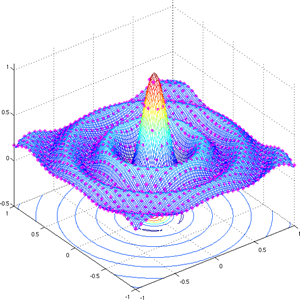
\includegraphics[scale=0.25]{../../img/sinc.PNG}}

\section{伴随}
\label{sec:org88be3ee}


\begin{definition}
设 \(T\in \mathcal{L}(V,W)\), \(T\)的伴随是满足如下条件的函数\(T^{*}:W\to V,\forall v\in V , \forall w\in W, \langle Tv,w \rangle = \langle v,T^{*}w \rangle\)
\end{definition}

为了检验上述定义的意义,我们假设\(\mathcal{L}(V,W)\), 并取定\(w\in W\),考虑\(V\)上将\(v\in V\)映射成\(\langle Tv,w \rangle\)的线性泛函,这个线性泛函依赖于\(T\)和\(w\)。由里斯表示定理,存在\(V\)中唯一一个向量使得该线性泛函是通过与该向量做内积得到的。我们将这个唯一的向量记为\(T^{*}w\),也就是说,\(T^{*}w\)是\(V\)中唯一一个满足下面条件的向量:对每个\(v\in V\)均有\(\langle Tv,w \rangle = \langle v,T^{*}w \rangle\)

\begin{tikzinstance}
定义\(T:\mathbf{R}^{3}\to \mathbf{R}^{2}\)为\(T(x_{1},x_{2},x_{3}) = (x_{2}+3x_{3},2x_{1})\) 求\(T^{*}\)

根据定义\(T^{*}\)是\(\mathbf{R}^{2}\)到\(\mathbf{R}^{3}\)的函数。要计算\(T^{*}\),取定一个点\((y_{1},y_{2})\in \mathbf{R}^{2}\),那么对于每个\((x_{1},x_{2},x_{3})\in \mathbf{R}^{3}\)有:
\begin{eqnarray}
\label{eq:1}
\langle (x_{1},x_{2},x_{3}),T^{*}(y_{1},y_{2}) \rangle &=& \langle T(x_{1},x_{2},x_{3}),(y_{1},y_{2}) \rangle \\
&=& \langle (x_{2}+3x_{3},2x_{1},(y_{1},y_{2}) \rangle \\
&=& x_{2}y_{1} + 3x_{3}y_{1} + 2x_{1}y_{2} \\
&=& \langle (x_{1},x_{2},x_{3}) , (2y_{2},y_{1},3y_{1}) \rangle
\end{eqnarray}
于是,\(T^{*}(y_{1},y_{2}) = (2y_{2},y_{1},3y_{1})\)
\end{tikzinstance}

\begin{tikzinstance}
取定\(u\in V\)和\(x\in W\),定义\(T\in \mathcal{L}(V,W)\)如下:对每个\(v\in V\)有\(Tv = \langle v,u \rangle x\),求\(T^{*}\)

根据定义:
\begin{eqnarray}
\label{eq:2}
 \langle Tv,w \rangle  &=& \langle  \langle v,u \rangle x , w\rangle  \\
&=& \langle v,u \rangle \langle x,w \rangle \\
&=& \langle v,\langle w,x \rangle u  \rangle
\end{eqnarray}

所以,\(T^{*}w = \langle w,x \rangle u\)
\end{tikzinstance}
注意,在上面两个例子中\(T^{*}\)不只是函数而且还是线性映射。
\begin{tikztheorem}
若\(T\in \mathcal{L}(V,W)\),则\(T^{*}\in \mathcal{L}(W,V)\)
\end{tikztheorem}
\begin{tikzproof}
设\(T\in \mathcal{L}(V,W)\),取定\(w_{1},w_{2}\in W\),若\(v\in V\),则:
\begin{eqnarray}
\label{eq:4}
 \langle v,T^{*}(w_{1} + w_{2}) \rangle  &=& \langle Tv,w_{1}+w_{2} \rangle  \\
&=& \langle Tv,w_{1} \rangle + \langle Tv,w_{2} \rangle \\
&=& \langle v,T^{*}(w_{1}) \rangle  + \langle v,T^{*}W_{2} \rangle  \\
&=& \langle v,T^{*}w_{1} + T^{*}w_{2} \rangle
\end{eqnarray}
即,\(T^{*(w_{1} + w_{2})} = T^{*}w_{1} + T^{*}w_{2}\)
\end{tikzproof}
另一方面,若\(\lambda\in \mathbf{F},w\in W\),则:
\begin{eqnarray}
\label{eq:5}
\langle v,T^{*}(\lambda w) \rangle  &=& \langle Tv,\lambda w \rangle   \\
&=& \bar{\lambda} \langle Tv,w \rangle \\
&=& \bar{\lambda} \langle v,T^{*}w \rangle \\
&=& \langle v,\lambda T^{*}w \rangle
\end{eqnarray}
即,\(T^{*}(\lambda w) = \lambda T^{*} w\).
因此\(T^{*}\)是线性映射。

伴随的性质:
\begin{tikztheorem}
\begin{enumerate}
\item 对所有\(S,T\in \mathcal{L}(V,W)\)均有\((S+T)^{*} = S^{*} + T^{*}\)
\item 对所有\(T\in \mathcal{L}(V,W),\lambda\in \mathbf{F}\)均有\((\lambda T)^{*} = \bar{\lambda}T^{*}\)
\item 对所有\(T\in \mathcal{L}(V,W)\),均有\((T^{*})^{*} = T\)
\item \(I^{*} = I\),这里\(I\)是\(V\)上的恒等算子
\item 对所有\(T\in \mathcal{L}(V,W)\)和\(S\in \mathcal{L}(V,W)\)均有\((ST)^{*} = T^{*}S^{*}\)
\end{enumerate}
\end{tikztheorem}

\begin{proof}
对于 a 有:
\begin{eqnarray}
\label{eq:3}
\langle v,(S+T)^{*}w \rangle  &=& \langle (S+T)v,w \rangle  \\
&=& \langle Sv,w \rangle  + \langle Tv,w \rangle \\
&=& \langle v,S^{*}w \rangle + \langle v,T^{*}w \rangle \\
&=& \langle v,S^{*}w + T^{*}w \rangle
\end{eqnarray}
即有:\((S+T)^{*}w = S^{*}w + T^{*}w\)

对于 b 有:
\begin{eqnarray}
\label{eq:6}
\langle v,(\lambda T)^{*}w \rangle  &=& \langle \lambda T v,w \rangle  \\
&=&\lambda \langle Tv,w \rangle \\
&=& \lambda \langle v,T^{*}w \rangle \\
&=& \langle v,\bar{\lambda}T^{*}w \rangle
\end{eqnarray}
即有:\((\lambda T)^{*} = \bar{\lambda}T^{*}\)

对于 c 有:
\begin{eqnarray}
\label{eq:7}
\langle w,(T^{*})^{*} v \rangle  &=& \langle T^{*}w,v \rangle = \bar{ \langle v,T^{*}w \rangle  }  =\bar{ \langle Tv, w \rangle  } = \langle w,Tv \rangle  \\
\end{eqnarray}
所以,\((T^{*})^{*} v = Tv\)

对于 d 有:
\begin{equation}
\label{eq:8}
\langle v,I^{*}u \rangle = \langle Iv,u \rangle  = \langle v,u \rangle = \langle v,Iu \rangle
\end{equation}

对于 e 有:
\begin{equation}
\label{eq:9}
\langle v,(ST)^{*}u \rangle = \langle STv,u \rangle = \langle Tv,S^{*}u \rangle = \langle v,T^{*}(S^{*}u) \rangle
\end{equation}
即有:\((ST)^{*}u = T^{*}S^{*}u\)
\end{proof}

接下来,我们阐述线性映射及其伴随的零空间和值域之间的关系。
\begin{tikztheorem}
设\(T\in \mathcal{L}(V,W)\),则:
\begin{enumerate}
\item \(\mathrm{null} T^{*} = (\mathrm{range}T)^{\bot}\)
\item \(\mathrm{range}T^{*} = (\mathrm{null}T)^{\bot}\)
\item \(\mathrm{null}T = (\mathrm{range}T^{*})^{\bot}\)
\item \(\mathrm{range}T = (\mathrm{null}T^{*})^{\bot}\)
\end{enumerate}
\end{tikztheorem}
\begin{tikzproof}
\(\forall w \in W\),\(w\in \mathrm{null}T^{*}\),则:

\begin{eqnarray}
\label{eq:10}
w\in \mathrm{null}T^{*}&\Leftrightarrow&T^{*}w = 0 \\
&\Leftrightarrow & \langle v,T^{*}w \rangle \qquad \forall v\in V \\
&\Leftrightarrow& \langle Tv,w \rangle =0 \qquad \forall v\in V \\
&\Leftrightarrow& w\in \mathrm{range}T^{\bot}
\end{eqnarray}
于是,\(\mathrm{null}T^{*} = ( \mathrm{range}T )^{\bot}\)
\end{tikzproof}

\begin{definition}
\(m\times n\)矩阵的共轭转置是先互换行和列,然后再对每个元素取共轭得到的\(n\times m\)矩阵。
\end{definition}
\begin{tikztheorem}
设\(T\in \mathcal{L}(V,W)\),假设\(e_{1},\ldots ,e_{n}\)是\(V\)的规范正交基,\(f_{1},\ldots ,f_{m}\)是\(W\)的规范正交基。则\(\mathcal{M}(T^{*},(f_{1},\ldots ,f_{m}),(e_{1},\ldots ,e_{n}))\)是\(\mathcal{M}\)
\end{tikztheorem}

\begin{tikzproof}
把\(Te_{k}\)写成\(f_{j}\)的线性组合可以得到\(\mathcal{M}(T)\)的第\(k\)列,在这个线性组合中用到的标量系数构成了\(\mathcal{M}(T)\)的第\(k\)列,因为\(f_{1},\ldots ,f_{m}\)是\(W\)的规范正交基,所以:
\begin{equation}
\label{eq:11}
Te_{k} = \langle Te_{k},f_{1} \rangle f_{1} + \ldots + \langle T{e_{k}},f_{m} \rangle f_{m}
\end{equation}
于是\(\mathcal{M}(T)\)的第\(k\)列第\(j\)行的元素是\(\langle Te_{k},f_{j} \rangle\)
把\(T\)替换为\(T^{*}\),再互换\(e\)和\(f\),可以得到,\(\mathcal{M}^{*}(T)\)的第\(j\)行第\(k\)列元素为:\(\langle T^{*}f_{k}, e_{j} \rangle\),其等于\(\langle f_{k}, T e_{j} \rangle = \bar{ \langle Te_{j},f_{k} \rangle  }\),这又是\(\mathcal{M}(T)\)的对应元素的复共轭。也就是说\(\mathcal{M}(T)\)和\(\mathcal{M}(T^{*})\)之间是共轭转置的关系。
\end{tikzproof}
\section{自伴算子}
\label{sec:org3a59b79}


现在我们关注一下内积空间上的算子。
\begin{definition}
算子\(T\in \mathcal{L}(V)\)称为自伴的,如果\(T= T^{*}\).也就是说,\(T\in \mathcal{L}(V)\)是自伴的当且仅当\(\langle Tv,w \rangle = \langle v,Tw \rangle  ,\forall v,w\in V\)
\end{definition}
自伴意味着:\(\mathcal{M}(T) = \mathcal{M}(T^{*})\),伴随在\(\mathcal{L}(V)\)上起的作用犹如复共轭在\(\mathcal{C}\)上起的作用。复数\(z\)是实的当且仅当\(z=\bar{z}\),因此自伴算子可以与实数类比。自伴意味着实对称矩阵。接下来我们证明实对称矩阵的特征值都是实数。

\begin{tikztheorem}
自伴算子的每个特征值都是实数。
\end{tikztheorem}
\begin{tikzproof}
设\(T\)是\(V\)上的自伴算子,\(\lambda\)是\(T\)的本征值,\(v\)是\(V\)中的非零向量使得\(Tv= \lambda v\),则:
\begin{eqnarray}
\label{eq:15}
\lambda \lvert v \rvert^{2} &=& \langle \lambda v,v \rangle \\
&=& \langle Tv,v \rangle \\
&=& \langle v,Tv \rangle \\
&=& \langle v,\lambda v \rangle  \\
&=& \bar{\lambda} \langle v,v \rangle \\
&=& \bar{\lambda} \lvert v \rvert^{2}
\end{eqnarray}



于是,\(\lambda = \bar{\lambda}\),即\(\lambda\)是实的。
\end{tikzproof}

\begin{tikztheorem}
在\(\mathbf{C}\)上,只有\(\mathbf{0}\)算子才能使\(Tv\)总正交于\(v\)。设\(V\)是复内积空间,\(T\in \mathcal{L}(V)\)。假设对所有\(v\in V\)均有\(\langle Tv,v \rangle = 0\),则\(T=0\)
\end{tikztheorem}

\begin{tikztheorem}
在\(\mathbf{C}\)上,仅自伴算子才能使\(\langle Tv,v \rangle\)都是实数。设\(V\)是复内积空间,\(T\in \mathcal{L}(V)\)。则\(T\)是自伴的当且仅当对每个\(v\in V\)均有\(\langle Tv,v \rangle \in \mathbf{R}\)
\end{tikztheorem}
\begin{proof}
设\(v\in V\),则:
\begin{equation}
\label{eq:13}
\langle Tv,v \rangle - \bar{ \langle Tv,v \rangle  } = \langle Tv,v \rangle - \langle v,Tv \rangle = \langle Tv,v \rangle - \langle T^{*}v,v \rangle = \langle (T- T^{*})v,v \rangle
\end{equation}
若对每个\(v\in V\)均有\(\langle Tv,v \rangle \in \mathbf{R}\),则必有\(T-T^{*}\)是\(\mathbf{0}\)算子。
反之,若\(T\)是自伴的,则上式右端等于 0。所以\(\forall v\in V\),均有\(\langle Tv,v \rangle = \bar{\langle Tv,v \rangle}\),即\(\langle Tv,v \rangle\in \mathbf{R}\)
\end{proof}
\begin{tikztheorem}
若\(T\)是\(V\)上的自伴算子使得对于所有\(v\in V\)均有\(\langle Tv,v \rangle  = 0\),则\(T=0\)
\end{tikztheorem}
\begin{proof}
假设\(V\)是实内积空间,若\(u,w\in V\),则:
\begin{equation}
\label{eq:14}
\langle Tu,w \rangle  = \frac{ \langle T(u+w),u+w \rangle  - \langle T(u-w),(u-w) \rangle  }{4}
\end{equation}
因为\(\langle T(u+w),(u+w) \rangle\) 和 \(\langle T(u-w),(u-w) \rangle\) 都是\(\langle Tv,v \rangle\)的形式,所以\(\langle Tu,w \rangle =0\),又由于\(u,w\)的任意性,则\(T=0\)
\end{proof}
\section{正规算子}
\label{sec:org13b436a}


\begin{definition}
内积空间上的算子称为正规的,如果它和它的伴随是交换的。也就是说,\(T\in \mathcal{L}(V)\)是正规的,如果\(T^{*}T=TT^{*}\)
\end{definition}
注意一个算子如果是自伴的,那么\(T=T^{*}\);如果是正规的,那么\(T^{*}T = TT^{*}\)。所以一个算子可以是正规的但不是自伴的。但是一个算子是自伴的肯定是正规的。

\begin{tikztheorem}
算子\(T\in \mathcal{L}(V)\)是正规的当且仅当对所有\(v\in V\)均有\(\lVert Tv \rVert = \lVert T^{*}v \rVert\)
\end{tikztheorem}
\begin{proof}
设\(T\in \mathcal{L}(V)\):
\begin{eqnarray}
\label{eq:16}
TT^{*} - T^{*}T = 0&\Leftrightarrow& \langle (TT^{*} - T^{*}T )v,v \rangle =0 \\
&\Leftrightarrow& \langle TT^{*}v,v \rangle = \langle T^{*}Tv,v \rangle \\
&\Leftrightarrow& \langle T^{*}v,T^{*}v \rangle = \langle Tv,Tv \rangle
\end{eqnarray}
\end{proof}
\begin{tikztheorem}
设\(T\in \mathcal{L}(V)\)是正规的,且\(v\in V\)是\(T\)的相应于本征值\(\lambda\)的特征向量,则\(v\)也是\(T^{*}\)相应于\(\bar{\lambda}\)的本征向量
\end{tikztheorem}
\begin{proof}
因为\(T\)是正规的,所以\(T-\lambda I\)也是正规的。所以:
\begin{equation}
\label{eq:17}
0= \lVert (T-\lambda I)v \rVert = \lVert (T-\lambda I)^{*} v \rVert = \lVert (T^{*} - \bar{\lambda}I^{*})v \rVert
\end{equation}
\end{proof}
\begin{tikztheorem}
设\(T\in \mathcal{L}(V)\)是正规的,则\(T\)的相应于不同本征值的本征向量是正交的。
\end{tikztheorem}
\begin{proof}
设\(\alpha,\beta\)是\(T\)的不同本征值,\(u,v\)分别是相应的本征向量,于是\(Tu=\alpha u\)且\(Tv = \beta v\)。因此:
\begin{eqnarray}
\label{eq:18}
(\alpha - \beta) \langle u,v \rangle  &=& \langle au,v \rangle - \langle u,\bar{\beta}v \rangle  \\
&=& \langle Tu,v \rangle - \langle u,T^{*}v \rangle \\
&=& 0
\end{eqnarray}
因为\(\alpha \neq \beta\),上面的等式表明\(\langle u,v \rangle =0\)。因此\(u\)和\(v\)是正交的。
\end{proof}
\section{总结}
\label{sec:orgd8f3384}


自伴和正规都是针对内积空间上的算子而言,算子是自身到自身的线性映射。自伴算子对应的矩阵是实对称的。起对应的特征向量是实数。正规的算子,其伴随是可交换的,但是正规算子不一定是自伴的。
\end{document}
